% !TeX root = ../main.tex

\section{L'analyse des données}
Une des premières tâches que j'ai effectuées a été que recalculée à partir des données brutes récoltées sur chaque slab, la production mensuelle des différentes fosses de Somaïr. Pour cela, j'ai eu accès  à la data-plateforme d’Orano qui est hébergé sur Dataiku. 

Dataiku est une plateforme conçue pour simplifier et démocratiser l'analyse de donnée. Pour cela, il n'y a même pas besoin d'écrire une ligne de code, car Dataiku a des recettes visuelles. Pour ceux qui souhaitent aller plus loin, il est possible d'écrire des recettes en python ou en R. Pour effectuer mes analyses, je me suis plutôt appuyé sur les recettes Python qui exploitent la librairie \href{https://pandas.pydata.org/}{Pandas} et \href{https://numpy.org/}{Numpy}.

Les données en provenance de la CanOp ont d'abord besoin d'être nettoyées, car il y a parfois des problèmes de mesure, des bugs et l'opérateur a la possibilité de supprimer une mesure, mais cette fonctionnalité est implémentée de telle manière que la mesure est toujours présente, mais avec une valeur de -1. Il faut donc supprimer toutes ces valeurs. J'ai également eu une colonne ne contenant que des numéros, mais dont certains étaient sauvés comme des strings et d'autre comme des int.

J'ai ensuite pu établir les teneurs en uranium de chaque slab en utilisant la formule suivante\footnote{Les cps sont des choc par seconde, soit le nombre de photon qui sont rentre en colition avec le crystal}~:
\[
    \text{Teneur en uranium} = 
    \begin{cases}
        cps_{\text{ sonde base}} \times 0.0002 \\
        cps_{\text{ sonde haut}} \times 0.0011
    \end{cases}
\]


\begin{figure}
    \centering
    \begin{subfigure}{0.45\textwidth}
        \centering
        \frame{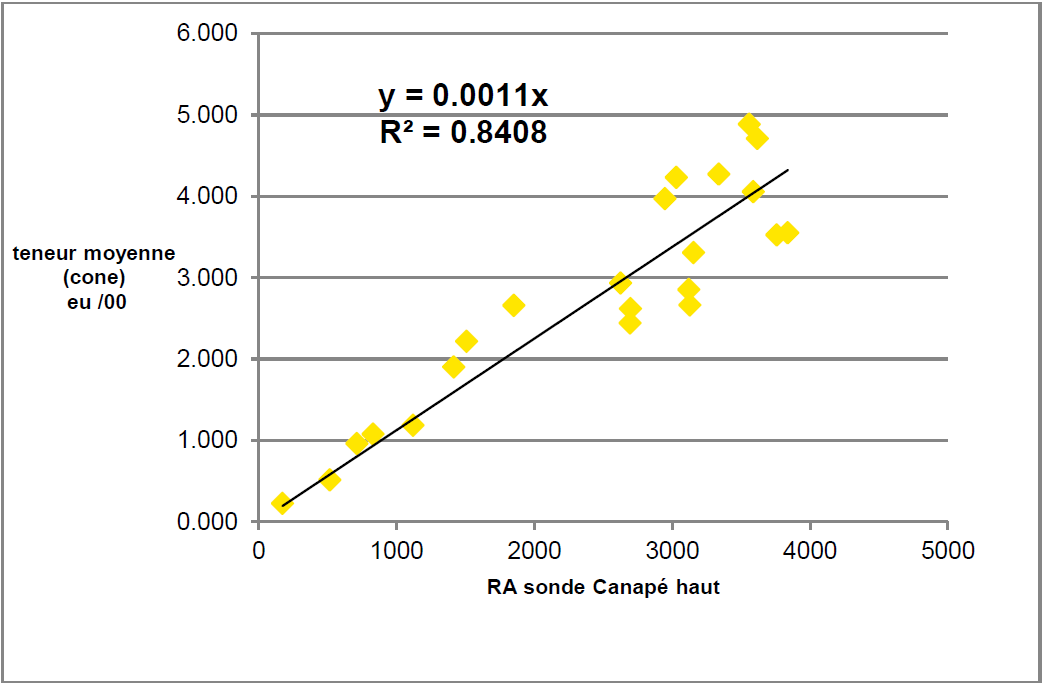
\includegraphics[width=\textwidth,trim=4 1cm 4 5,clip]{img/graph/Correlation_sonde_haute.png}}
        \caption{Corrélation pour la sonde haute}
        \label{fig_correlation_sonde_haute}
    \end{subfigure}
    \begin{subfigure}{0.45\textwidth}
        \centering
        \frame{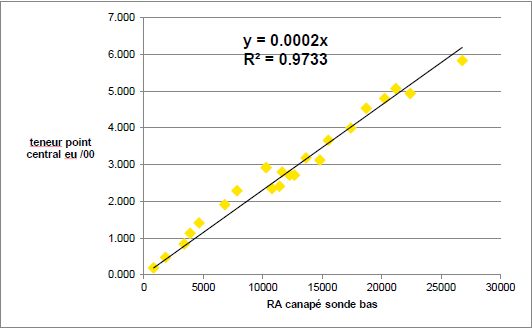
\includegraphics[width=\textwidth,trim=4 4 4 4,clip]{img/graph/Correlation_sonde_basse.png}}
        \caption{Corrélation pour la sonde basse}
        \label{fig_correlation_sonde_basse}
    \end{subfigure}
    \caption[Corrélation entre la radiométrie et la teneur d'uranium]{Corrélation entre la radiométrie et la teneur d'uranium pour les sondes haute et basse, Source~: Compte-rendu de mission Orano, Réf.~: IDF-CR-001714}
    \label{fig_correlation_sonde}
\end{figure}
Ces corrélations on était obtenu directement dans la fosse de Somaïr avec des mesures empiriques (voir \cref{fig_correlation_sonde}).

À partir des teneurs en uranium, j'ai pu repartir les slabs et les chargements des différents camions dans leur différente classe (voir\ref{}). Une fois les chargements repartis, j'ai pu calculer la production mensuelle de chaque fosse en tenant compte de comment est fait le reporting de la production. En effet, la production est calculée du 26 du mois précédent au 25 du mois actuel sauf pour les mois de décembre/janvier et de juin/juillet ou la date limite est le 1er~janvier/juillet à 5h. C'est là une autre subtilité qui est présente chaque mois auquel j'ai dû faire face, car la mine ne souhaite pas scinder en 2 la production de l'équipe de nuit (21h-5h).